\documentclass[11pt]{article}
\usepackage[margin=1in]{geometry}
\usepackage{graphicx}
\usepackage{listings}
\usepackage{amsmath}
\usepackage{color}
\usepackage{caption} % Required for \captionof
\usepackage{float}
\usepackage{hyperref}
\usepackage{tikz}
\usetikzlibrary{shapes.geometric, arrows.meta, positioning}
\usepackage{adjustbox} % For better scaling control

\hypersetup{
    colorlinks=true,
    linkcolor=blue,
    citecolor=blue,
    filecolor=blue,
    urlcolor=blue
}

% Unified TikZ styles for all diagrams
\tikzset{
    block/.style={rectangle, draw=black, fill=blue!20, text centered, rounded corners, minimum height=2em, minimum width=4em, font=\small},
    arrow/.style={thick, ->, >=stealth},
    startstop/.style={rectangle, rounded corners, minimum width=2.5cm, minimum height=0.8cm, text centered, draw=black, fill=gray!20, font=\small},
    process/.style={rectangle, minimum width=2.5cm, minimum height=0.8cm, text centered, draw=black, fill=blue!10, font=\small},
    decision/.style={diamond, aspect=1.5, minimum width=2.5cm, minimum height=0.8cm, text centered, draw=black, fill=orange!10, font=\small}
}

\title{COL 216 Assignment 3: \\ L1 Cache Simulator for Quad-Core Processor}
\author{Aditya Anand (2023CS50284) \\ Vansh Ramani (2023CS50804)}
\date{May 9, 2025}

\begin{document}

\maketitle

\section{Implementation}

\subsection{Class Overview}
The simulator comprises six key modules, each handling a specific aspect of the L1 cache simulation:

\begin{itemize}
    \item \textbf{TraceReader}: Reads and parses memory access traces for each core.
    \item \textbf{Core}: Simulates a processor core’s execution, issuing memory instructions and managing stalls.
    \item \textbf{Cache}: Models a private, E-way set-associative L1 data cache per core with $2^s$ sets and $2^b$-byte blocks. Supports write-back, write-allocate, LRU replacement, and MESI coherence.
    \item \textbf{Bus}: A shared communication medium handling coherence transactions and arbitration.
    \item \textbf{Simulator}: Orchestrates core execution, bus activity, and simulation cycles.
    \item \textbf{StatsPrinter}: Aggregates and reports cache performance metrics.
\end{itemize}

\subsection{Module Descriptions}

\subsubsection{TraceReader}
Reads trace files (one per core) line-by-line. Each line specifies a memory operation (R or W) and a hexadecimal address, converted into \texttt{TraceEntry} structs with a 32-bit address and operation type. Uses standard C++ I/O with input validation.

\subsubsection{Core}
Represents a CPU core, executing one memory operation per cycle unless stalled. Communicates with its private L1 cache and other caches via the bus. Features:
\begin{itemize}
    \item Instruction stream from the trace.
    \item Counters for instructions, read/write operations, idle cycles, and total cycles.
    \item State tracking for stalls due to cache misses or coherence waits.
    \item \texttt{tick()} function to issue instructions or increment idle time.
\end{itemize}

\subsubsection{Cache}
Each core has a local cache configured with:
\begin{itemize}
    \item $E$ lines per set, $2^s$ sets, and block size of $2^b$ bytes.
    \item Cache lines storing tags, MESI states, LRU timestamps, valid/dirty flags.
    \item Read/write methods updating LRU order on hits and initiating coherence on misses.
    \item \texttt{allocateBlock()} and \texttt{handleMiss()} for block allocation and evictions.
    \item Snooping support for BusRd, BusRdX, and MESI transitions (e.g., Shared $\to$ Invalid).
\end{itemize}

\subsubsection{Bus}
Manages inter-cache coherence communication:
\begin{itemize}
    \item Round-robin arbitration for transactions.
    \item Queues for pending transactions, prioritizing BusRdX over BusRd or WriteBack.
    \item \texttt{tick()} processes transactions, handles snoop responses, and triggers cache state changes.
    \item Tracks bytes transferred and latency for memory vs. cache-to-cache transfers.
\end{itemize}

\subsubsection{Simulator}
Coordinates cores and caches. In each cycle:
\begin{itemize}
    \item Calls \texttt{tick()} on each core.
    \item Updates the bus and processes snoop responses.
    \item Monitors termination when all cores finish their traces.
    \item Finalizes per-core cycle counts and statistics.
\end{itemize}

\subsubsection{StatsPrinter}
Reports:
\begin{itemize}
    \item Cache parameters (size, associativity, block size).
    \item Per-core stats: accesses, execution/idle cycles, misses, evictions, writebacks, invalidations.
    \item Bus stats: total transactions and data transferred.
\end{itemize}

\begin{figure}[H]
\centering
\begin{adjustbox}{max width=\textwidth}
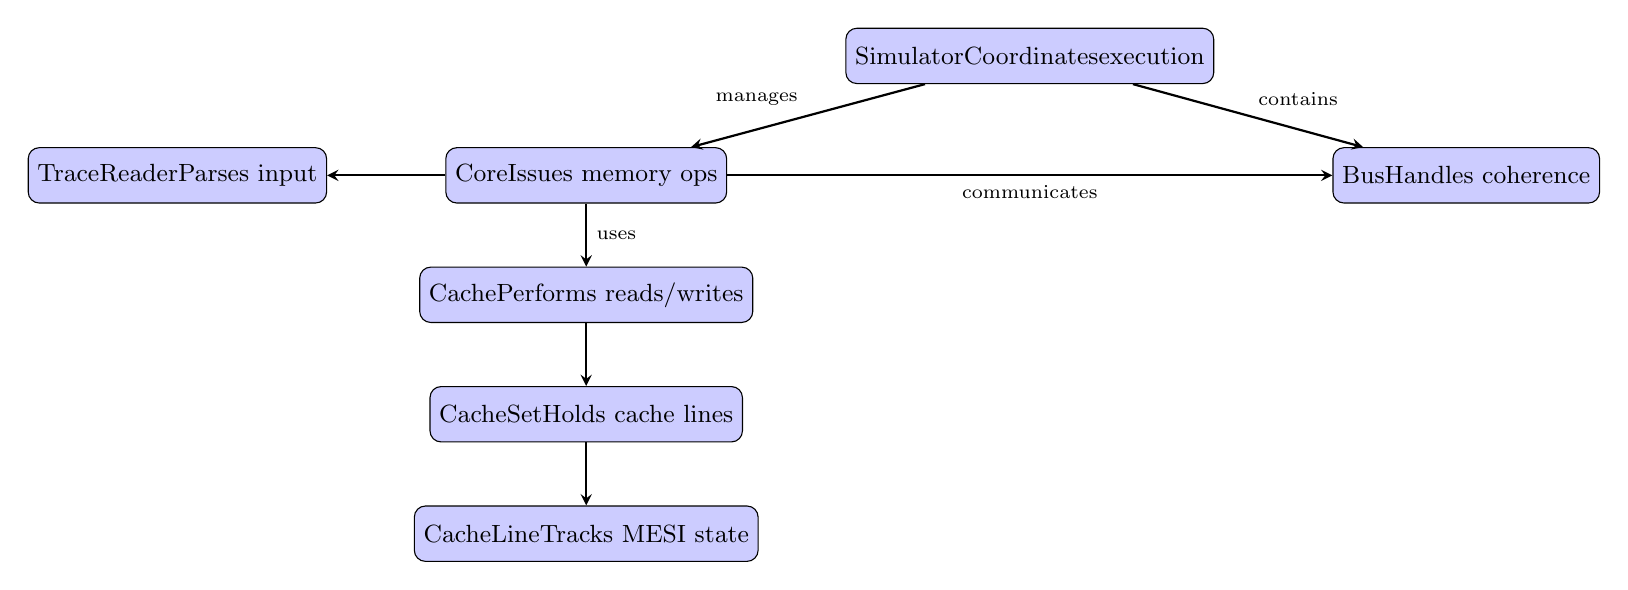
\begin{tikzpicture}[node distance=0.8cm and 1.5cm]
    % Nodes
    \node (simulator) [block] {Simulator\\Coordinates\\execution};
    \node (core) [block, below left=of simulator] {Core\\Issues memory ops};
    \node (bus) [block, below right=of simulator] {Bus\\Handles coherence};
    \node (cache) [block, below=of core] {Cache\\Performs reads/writes};
    \node (set) [block, below=of cache] {CacheSet\\Holds cache lines};
    \node (line) [block, below=of set] {CacheLine\\Tracks MESI state};
    \node (reader) [block, left=of core] {TraceReader\\Parses input};
    % Arrows
    \draw [arrow] (simulator) -- node[midway, above left, font=\scriptsize] {manages} (core);
    \draw [arrow] (simulator) -- node[midway, above right, font=\scriptsize] {contains} (bus);
    \draw [arrow] (core) -- node[midway, right, font=\scriptsize] {uses} (cache);
    \draw [arrow] (cache) -- (set);
    \draw [arrow] (set) -- (line);
    \draw [arrow] (core) -- node[midway, below, font=\scriptsize] {communicates} (bus);
    \draw [arrow] (core) -- (reader);
\end{tikzpicture}
\end{adjustbox}
\caption{Class interaction diagram of the L1 Cache Simulator}
\end{figure}

\section{Data Structures}

Core data structures include:
\begin{itemize}
    \item \textbf{CacheLine}: Stores \texttt{tag}, \texttt{flags.valid}, \texttt{flags.state} (MESI), \texttt{lastUsedCycle} for LRU.
    \item \textbf{CacheSet}: \texttt{std::vector<CacheLine>} for lines, \texttt{std::unordered_map} for tag lookups.
    \item \textbf{MESI State} (Enum \texttt{CacheLineState}): MODIFIED, EXCLUSIVE, SHARED, INVALID.
    \item \textbf{BusRequestType} (Enum): BusRd, BusRdX, WriteBack.
    \item \textbf{BusTransaction}: \texttt{requesterId}, \texttt{address}, \texttt{type}, \texttt{startCycle}, \texttt{completionCycle}, \texttt{servedByCache}.
    \item \textbf{TraceEntry}: \texttt{op} (READ/WRITE), \texttt{addr} (32-bit).
    \item \textbf{Statistics}: Counters for hits, misses, evictions, writebacks, invalidations, idle cycles, instruction count, total cycles.
\end{itemize}

\begin{figure}[H]
\centering
\begin{adjustbox}{max width=\textwidth}
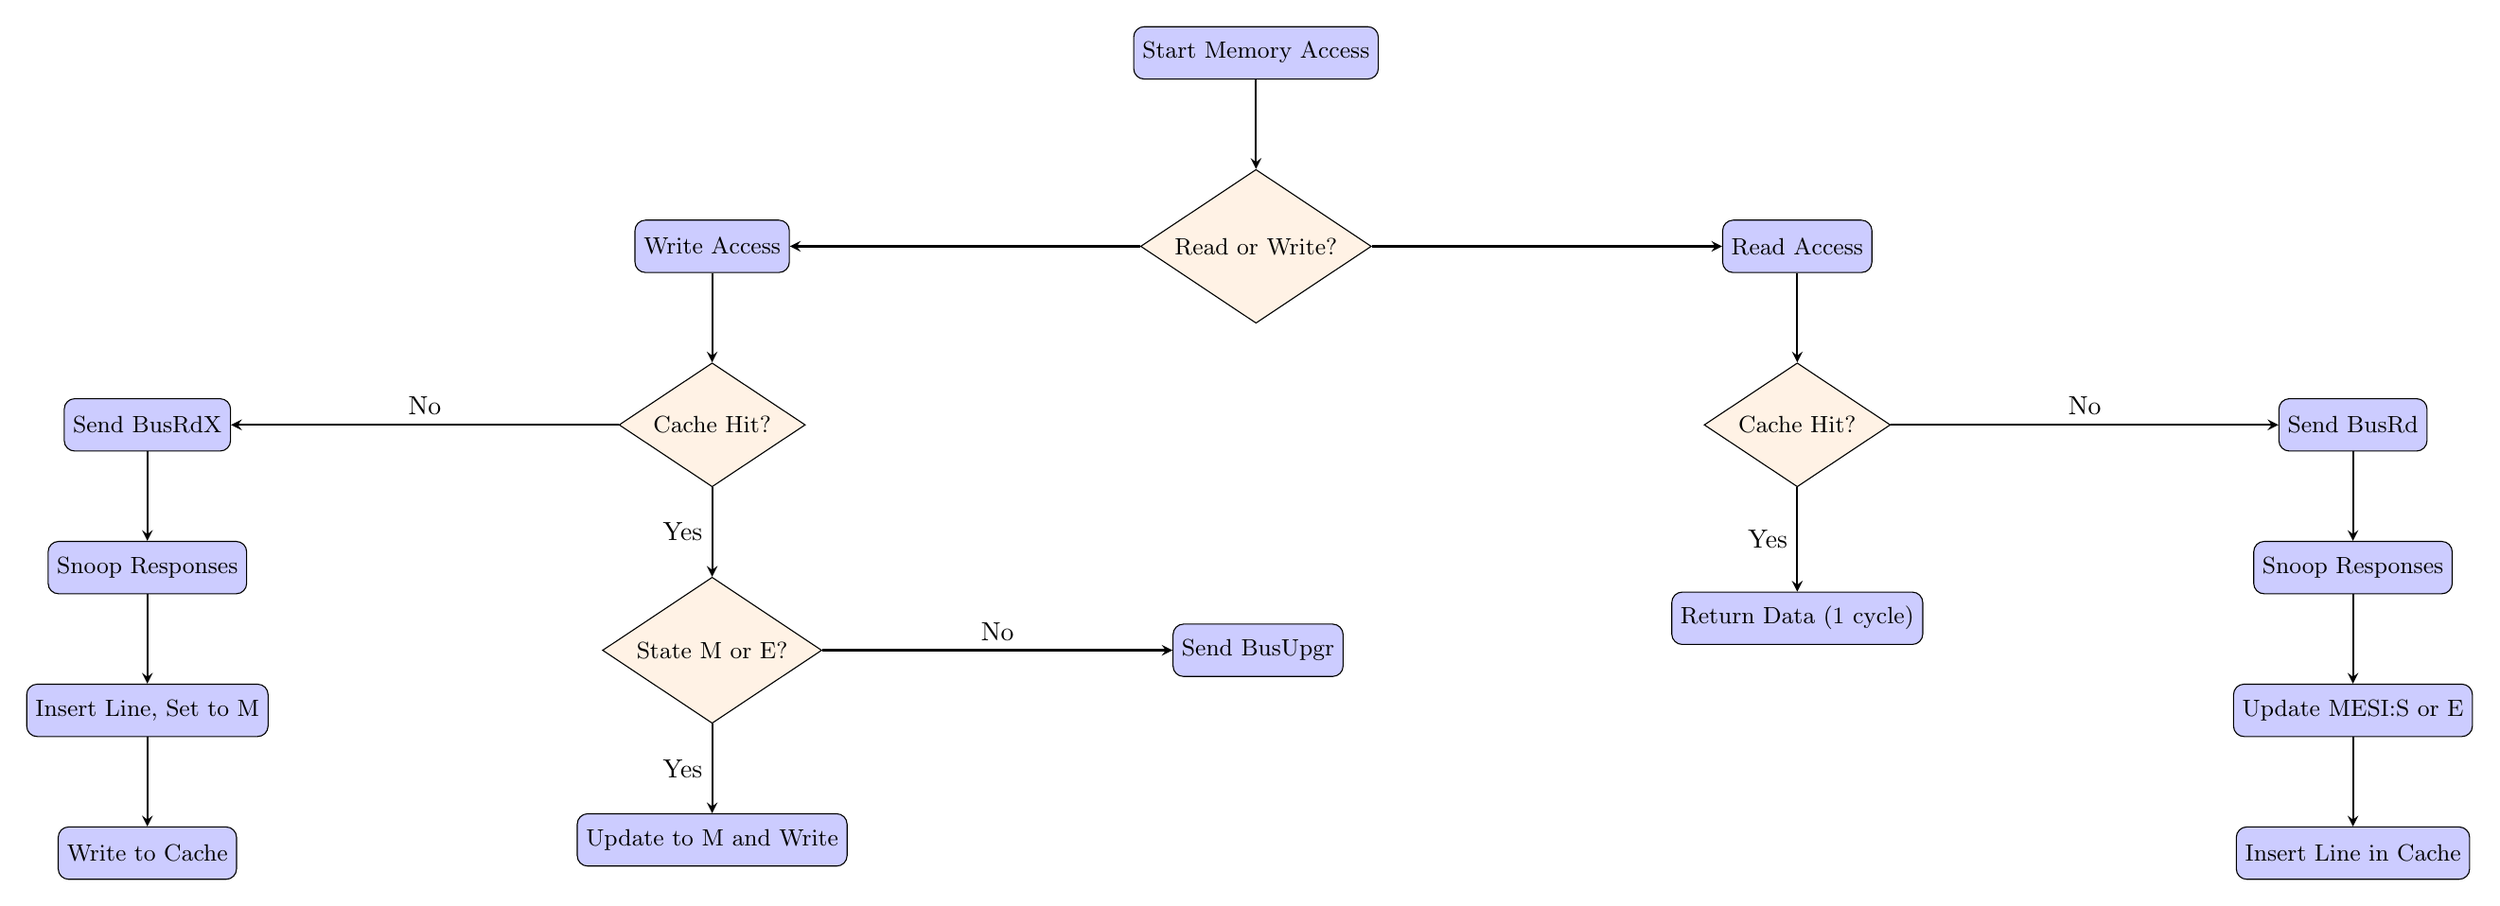
\begin{tikzpicture}[node distance=1.2cm and 1.2cm]
    % Start
    \node (start) [block] {Start Memory Access};
    % Access Type
    \node (access) [decision, below=of start] {Read or Write?};
    \node (read_hit) [block, right=of access, xshift=3.5cm] {Read Access};
    \node (write_hit) [block, left=of access, xshift=-3.5cm] {Write Access};
    % Read Path
    \node (read_hit_check) [decision, below=of read_hit] {Cache Hit?};
    \node (read_hit_ok) [block, below=of read_hit_check, yshift=-0.2cm] {Return Data (1 cycle)};
    \node (read_miss) [block, right=of read_hit_check, xshift=4cm] {Send BusRd};
    \node (read_snoop) [block, below=of read_miss] {Snoop Responses};
    \node (read_update) [block, below=of read_snoop] {Update MESI: \\ S or E};
    \node (read_insert) [block, below=of read_update] {Insert Line in Cache};
    % Write Path
    \node (write_hit_check) [decision, below=of write_hit] {Cache Hit?};
    \node (write_hit_mesistate) [decision, below=of write_hit_check] {State M or E?};
    \node (write_no_upgr) [block, right=of write_hit_mesistate, xshift=3.5cm] {Send BusUpgr};
    \node (write_update_M) [block, below=of write_hit_mesistate] {Update to M and Write};
    \node (write_miss) [block, left=of write_hit_check, xshift=-4cm] {Send BusRdX};
    \node (write_miss_snoop) [block, below=of write_miss] {Snoop Responses};
    \node (write_miss_update) [block, below=of write_miss_snoop] {Insert Line, Set to M};
    \node (write_miss_data) [block, below=of write_miss_update] {Write to Cache};
    % Arrows
    \draw [arrow] (start) -- (access);
    \draw [arrow] (access) -- (read_hit);
    \draw [arrow] (access) -- (write_hit);
    \draw [arrow] (read_hit) -- (read_hit_check);
    \draw [arrow] (read_hit_check) -- node[midway, left] {Yes} (read_hit_ok);
    \draw [arrow] (read_hit_check) -- node[midway, above] {No} (read_miss);
    \draw [arrow] (read_miss) -- (read_snoop);
    \draw [arrow] (read_snoop) -- (read_update);
    \draw [arrow] (read_update) -- (read_insert);
    \draw [arrow] (write_hit) -- (write_hit_check);
    \draw [arrow] (write_hit_check) -- node[midway, left] {Yes} (write_hit_mesistate);
    \draw [arrow] (write_hit_mesistate) -- node[midway, left] {Yes} (write_update_M);
    \draw [arrow] (write_hit_mesistate) -- node[midway, above] {No} (write_no_upgr);
    \draw [arrow] (write_hit_check) -- node[midway, above] {No} (write_miss);
    \draw [arrow] (write_miss) -- (write_miss_snoop);
    \draw [arrow] (write_miss_snoop) -- (write_miss_update);
    \draw [arrow] (write_miss_update) -- (write_miss_data);
\end{tikzpicture}
\end{adjustbox}
\caption{Memory access control flow for L1 cache simulator}
\end{figure}

\section{Control Flow Diagram}

\begin{figure}[H]
\centering
\begin{adjustbox}{max width=0.8\textwidth}
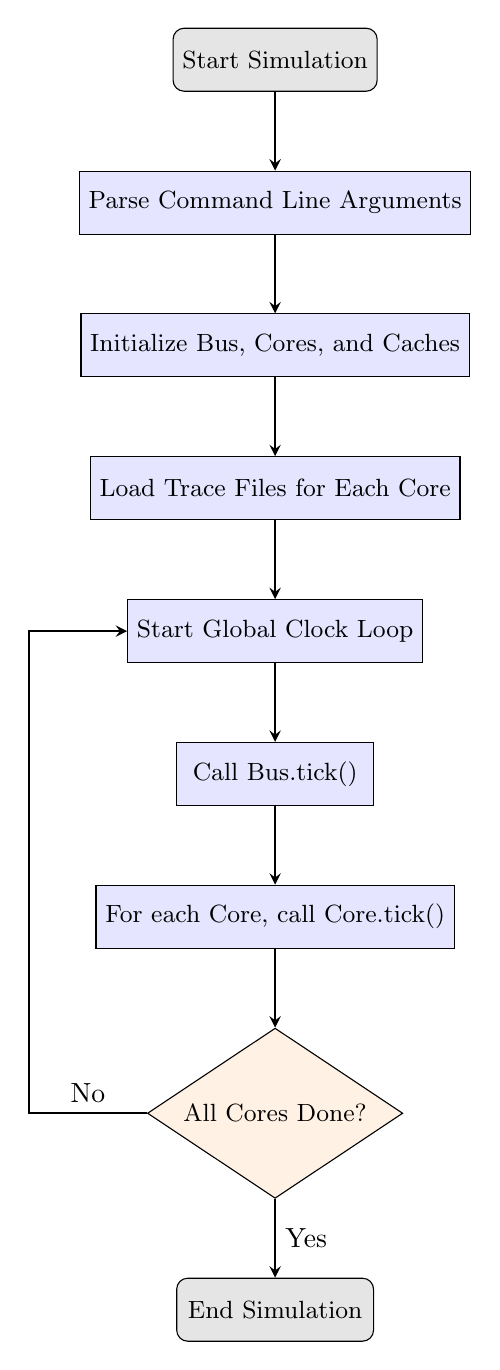
\begin{tikzpicture}[node distance=1cm and 1cm]
    % Nodes
    \node (start) [startstop] {Start Simulation};
    \node (args) [process, below=of start] {Parse Command Line Arguments};
    \node (init) [process, below=of args] {Initialize Bus, Cores, and Caches};
    \node (load) [process, below=of init] {Load Trace Files for Each Core};
    \node (loop) [process, below=of load] {Start Global Clock Loop};
    \node (busTick) [process, below=of loop] {Call Bus.tick()};
    \node (coreTick) [process, below=of busTick] {For each Core, call Core.tick()};
    \node (checkDone) [decision, below=of coreTick] {All Cores Done?};
    \node (done) [startstop, below=of checkDone] {End Simulation};
    % Arrows
    \draw [arrow] (start) -- (args);
    \draw [arrow] (args) -- (init);
    \draw [arrow] (init) -- (load);
    \draw [arrow] (load) -- (loop);
    \draw [arrow] (loop) -- (busTick);
    \draw [arrow] (busTick) -- (coreTick);
    \draw [arrow] (coreTick) -- (checkDone);
    \draw [arrow] (checkDone) -- node[right] {Yes} (done);
    \draw [arrow] (checkDone.west) -- ++(-1.5,0) node[midway, above] {No} |- (loop.west);
\end{tikzpicture}
\end{adjustbox}
\caption{Top-level global simulation control flow for L1 cache simulator}
\end{figure}

\section{Design Decisions}
The L1 cache simulator incorporates key design choices for realistic behavior, deterministic execution, and manageable complexity:

\begin{enumerate}
    \item \textbf{Idle Cycle Definition}: Idle cycles occur when a core waits for memory operations, including bus coherence or memory fetches. Total cycles = execution cycles + idle cycles.
    \item \textbf{MESI Protocol}: Implements full MESI with transitions:
        \begin{itemize}
            \item Shared $\to$ Modified: Issues BusRdX, triggers invalidations.
            \item Modified $\to$ Shared/Invalid: Via snooping on BusRd/BusRdX.
            \item Modified writebacks: 100-cycle latency.
        \end{itemize}
    \item \textbf{Writebacks}:
        \begin{itemize}
            \item Eviction: Synchronous writeback of dirty blocks.
            \item Snoop-triggered: Writeback before Modified $\to$ Shared/Invalid.
        \end{itemize}
    \item \textbf{Bus Arbitration}: One transaction at a time, prioritized:
        \begin{enumerate}
            \item BusUpgr (1 cycle).
            \item BusRdX, WriteBack.
            \item BusRd (lowest priority).
        \end{enumerate}
        Tie-breaking by ascending core ID.
    \item \textbf{Deterministic Core Order}: Cores 0–3 tick in fixed order for reproducibility.
    \item \textbf{Blocking Cache}: Core stalls on misses until transaction completes; caches respond to snoops in parallel.
    \item \textbf{Memory Latencies}:
        \begin{itemize}
            \item L1 hit: 1 cycle.
            \item Memory fetch: 100 cycles.
            \item Cache-to-cache: 2 cycles per 4-byte word.
            \item Writeback: 100 cycles.
        \end{itemize}
    \item \textbf{Cache Initialization}: All lines invalid at start (cold cache).
    \item \textbf{Word/Block Size}: 4-byte words, $2^b$-byte blocks.
    \item \textbf{Simplified Data}: Only tags, states, and timing modeled.
    \item \textbf{No Bus Pipelining}: One transaction at a time.
    \item \textbf{Microbenchmark Verification}: Validated MESI and writebacks with 2–5 instruction traces.
\end{enumerate}

\section{Performance Analysis}

To evaluate cache parameter impacts, we conducted experiments varying one parameter at a time while keeping others fixed at:
\begin{itemize}
    \item Number of sets: $2^s = 64$
    \item Associativity: $E = 2$
    \item Block size: $B = 32$ bytes
\end{itemize}

For each parameter, we doubled its value across runs and measured the \textbf{maximum execution cycles across all cores}, reflecting total workload completion time, including computation and stalls due to memory or coherence delays. Experiments used provided application traces, with results recorded for comparison.

\section{Implementation Challenges}

Key challenges encountered include:
\begin{enumerate}
    \item \textbf{Precise Cycle Synchronization}: Managing a global simulation loop while allowing independent core instruction issuance required careful delay handling for memory fetches, writebacks, and coherence events.
    \item \textbf{MESI State Coordination}: Ensuring correct MESI transitions across cores demanded rigorous tracking of local and remote operations, especially for Modified $\to$ Shared or Exclusive $\to$ Invalid transitions.
    \item \textbf{Bus Arbitration and Fairness}: Modeling realistic contention with deterministic behavior involved priority-based selection and round-robin tie-breaking.
    \item \textbf{Blocking Behavior and Stall Management}: Simulating blocking caches—halting cores on misses while responding to coherence requests—required separating execution from snoop handling and tracking core resumption.
    \item \textbf{Edge Case Handling}: Malformed trace files, invalid inputs, and misaligned addresses necessitated robust validation.
    \item \textbf{Comprehensive Metric Tracking}: Accurate tracking of idle cycles, evictions, writebacks, and data traffic required consistent counters across modules without double-counting.
\end{enumerate}

\section{Conclusion}

Our L1 cache simulator accurately models a quad-core processor with MESI coherence, write-back/write-allocate policy, and LRU eviction. It captures private cache and shared memory interactions, providing cycle-accurate statistics.

Key trends from parameter variation experiments:
\begin{enumerate}
    \item \textbf{Cache Size}: Larger caches reduce capacity and compulsory misses, but benefits plateau when the working set is fully accommodated.
    \item \textbf{Associativity}: Higher associativity (2-way or 4-way) reduces conflict misses, improving hit rates but potentially increasing access latency.
    \item \textbf{Block Size}: Balancing transfer time and spatial locality, block sizes of 32–64 bytes performed best for our traces.
\end{enumerate}

These results highlight cache architecture trade-offs and the importance of workload-specific configurations. The simulator enables functional validation and performance exploration in multicore systems.

\section{Repository}
Full source code and report: \\
\url{https://github.com/VanshRamani/CacheSim}

\end{document}